% !TeX root = main.tex
\chapter{Implementation}
\label{chap:implementation}

\newcommand{\impltagplain}[2]{\texorpdfstring{\textsuperscript{\textbf{\textcolor{#1}{[#2]}}}}{[#2]}}
\newcommand{\impltag}[3]{\texorpdfstring{\hyperlink{#1}{\textsuperscript{\textbf{\textcolor{#2}{[#3]}}}}}{[#3]}}
\newcommand{\impltaghead}[3]{\protect\hyperlink{#1}{\impltagplain{#2}{#3}}}
\newcommand{\runconf}{\impltag{implcomp:run}{darkblue}{run}}
\newcommand{\deployconf}{\impltag{implcomp:dep}{darkblue}{dep}}
\newcommand{\fedctlcli}{\impltag{implcomp:request}{paletteGreen}{cli}}
\newcommand{\submitsvc}{\impltag{implcomp:request}{paletteGreen}{svc}}
\newcommand{\regtag}{\impltag{implcomp:deploy}{paletteGreen}{reg}}
\newcommand{\nomadrenderer}{\impltag{implcomp:deploy}{paletteGreen}{nomad}}
\newcommand{\submitrunner}{\impltag{implcomp:deploy}{paletteGreen}{runner}}
\newcommand{\distroles}{\impltag{implcomp:runtime}{paletteOrange}{roles}}
\newcommand{\researchapp}{\impltag{implcomp:runtime}{paletteOrange}{app}}
\newcommand{\wandbtag}{\impltag{implcomp:observability}{gray}{wandb}}
\newcommand{\artifacttag}{\impltag{implcomp:observability}{gray}{art}}
\newcommand{\uilogstag}{\impltag{implcomp:observability}{gray}{ui}}
\newcommand{\substratetag}{\impltag{implcomp:substrate}{fedstalebrown}{cluster}}
\newcommand{\implterm}[2]{\textcolor{#1}{#2}}

This chapter has two parts. The first describes \texttt{fedctl}, the control path used to package, submit, deploy, monitor, and retrieve Flower experiments, and the dissertation-specific Flower application that implements the FL methods, tasks, and diagnostics evaluated in Chapter~\ref{chap:evaluation}. The second introduces \texttt{FedCover} (Sec.~\ref{sec:fedcover_impl}), the coverage-aware aggregation algorithm for asynchronous submodel FL.

The \texttt{fedctl} implementation follows the lifecycle of a run:
\[
\begin{aligned}
\begin{array}{@{}c@{}}\text{experiment specification}\\[-0.1em]\text{\small Sec.~\ref{sec:impl_configuration}}\end{array}
&\longrightarrow
\begin{array}{@{}c@{}}\text{packaging/submission}\\[-0.1em]\text{\small Secs.~\ref{sec:impl_configuration}, \ref{sec:impl_remote_execution}}\end{array}
\longrightarrow
\begin{array}{@{}c@{}}\text{cluster deployment}\\[-0.1em]\text{\small Sec.~\ref{sec:impl_remote_execution}}\end{array}
\\[0.85em]
&\longrightarrow
\begin{array}{@{}c@{}}\text{heterogeneity control}\\[-0.1em]\text{\small Sec.~\ref{sec:impl_heterogeneity_control}}\end{array}
\longrightarrow
\begin{array}{@{}c@{}}\text{method execution}\\[-0.1em]\text{\small Sec.~\ref{sec:impl_flower_application}}\end{array}
\longrightarrow
\begin{array}{@{}c@{}}\text{evidence}\\[-0.1em]\text{\small App.~\ref{appendix:observability_submit_ui}}\end{array}
\end{aligned}
\]

\FloatBarrier
\section{Overview of the \texttt{fedctl} System}
\label{sec:impl_overview}

The system separates cluster orchestration from experiment logic. \texttt{fedctl} is the orchestration layer: it packages a Flower application, renders the Nomad\footnote{Flower is the federated-learning framework used for these experiments and is widely used for FL work in the Computer Laboratory at the University of Cambridge. Nomad is the scheduler and orchestrator used to place runtime services on cluster machines. Appendix~\ref{def:flower} and Appendix~\ref{def:nomad} give the definitions.} jobs that place its services on the Raspberry Pi cluster, and preserves the resulting run evidence. \texttt{fedctl\_research} is the experiment layer, containing the tasks, methods, and diagnostics evaluated in Chapter~\ref{chap:evaluation}. This separation keeps execution conditions such as images, placement, service discovery, network shaping, logs, and artifacts separate from task construction, data partitioning, local training, evaluation, and aggregation.

\FloatBarrier
\subsection{System decomposition}
\label{sec:impl_main_components}

Figure~\ref{fig:fedctl_overview} is the component map for the implementation: specification, control plane, Flower runtime, and observability. 

\begin{figure}[!htbp]
\centering
\begin{tikzpicture}[
  >=Stealth,
  font=\scriptsize,
  arrow/.style={thick, ->},
  infraarrow/.style={thick, ->, dashed},
  coltitle/.style={font=\bfseries\small},
  groupbox/.style={draw, dashed, rounded corners=4pt, minimum width=3.0cm, minimum height=6.05cm, inner sep=0pt},
  cfggroup/.style={groupbox, fill=coreblue!8},
  ctlgroup/.style={groupbox, fill=paletteGreen!6},
  rungroup/.style={groupbox, fill=paletteOrange!6},
  obsgroup/.style={groupbox, fill=gray!6},
  innerbox/.style={draw, rounded corners=3pt, align=center, text width=2.25cm, minimum height=0.76cm, inner sep=3pt},
  cfgbox/.style={innerbox, fill=coreblue!28},
  ctlbox/.style={innerbox, fill=paletteGreen!18},
  runbox/.style={innerbox, fill=paletteOrange!20},
  obsbox/.style={innerbox, fill=gray!14},
  basebox/.style={draw, rounded corners=4pt, align=center, fill=white, text width=7.6cm, minimum height=0.85cm, inner sep=5pt}
]
\node[coltitle] at (0.0, 0.55) {Specification};
\node[coltitle] at (3.65, 0.55) {Control plane};
\node[coltitle] at (7.3, 0.55) {Flower runtime};
\node[coltitle] at (10.95, 0.55) {Observability};

\node[cfggroup] (config) at (0.0, -3.05) {};
\node[ctlgroup] (control) at (3.65, -3.05) {};
\node[rungroup] (runtime) at (7.3, -3.05) {};
\node[obsgroup] (observability) at (10.95, -3.05) {};

\node[cfgbox, anchor=north, minimum height=1.05cm] (spec) at (0.0, -0.3) {\textbf{Configuration}\\\runconf{} \deployconf};

\node[ctlbox, anchor=north] (cli) at (3.65, -0.3) {\textbf{\texttt{fedctl} CLI}\\\fedctlcli};
\node[ctlbox, anchor=north] (svc) at (3.65, -1.4) {\textbf{Submit service}\\\submitsvc};
\node[ctlbox, anchor=north] (reg) at (3.65, -2.5) {\textbf{Registry}\\\regtag};
\node[ctlbox, anchor=north] (nomad) at (3.65, -3.60) {\textbf{Nomad renderer}\\\nomadrenderer};
\node[ctlbox, anchor=north] (runner) at (3.65, -5.0) {\textbf{Submit runner}\\\submitrunner};

\node[runbox, anchor=north] (roles) at (7.3, -0.3) {\textbf{Distributed roles}\\\distroles};
\node[runbox, anchor=north] (app) at (7.3, -1.75) {\textbf{Research app}\\\researchapp};

\node[obsbox, anchor=north] (wandb) at (10.95, -0.3) {\textbf{W\&B}\\\wandbtag};
\node[obsbox, anchor=north] (art) at (10.95, -1.45) {\textbf{Structured artifacts}\\\artifacttag};
\node[obsbox, anchor=north] (ui) at (10.95, -2.9) {\textbf{Submit UI/logs}\\\uilogstag};

\node[basebox] (cluster) at (5.48, -7.32) {\textbf{Cluster substrate}\\\substratetag};

\draw[arrow] (config.east) -- (control.west);
\draw[arrow] (control.east) -- (runtime.west);
\draw[arrow] (runtime.east) -- (observability.west);
\draw[infraarrow] (cluster.north) -- ++(0,0.18) -| (control.south);
\draw[infraarrow] (cluster.north) -- ++(0,0.18) -| (runtime.south);
\end{tikzpicture}
\caption{\textbf{High-level \texttt{fedctl} execution stack.}}
\label{fig:fedctl_overview}
\end{figure}

\hypertarget{implcomp:run}{}\hypertarget{implcomp:dep}{}
\paragraph[Configuration.]{Configuration \impltaghead{implcomp:run}{darkblue}{run}\impltaghead{implcomp:dep}{darkblue}{dep}.\footnote{Throughout the following sections, superscript tags such as \textsuperscript{\textbf{\textcolor{darkblue}{[run]}}} identify the responsible component and link back to its explanatory paragraph.}}
Configuration covers both the application workload and the execution environment. The run side selects the FL method, task, partitioner, model-rate allocation, client sampling, local training budget, evaluation hooks, and random seed. The deployment side specifies typed workers, placement policy, resource reservations, registry and submit-service settings, and optional network profiles.

\hypertarget{implcomp:request}{}
\paragraph[Submission and admission control.]{Submission and admission control \impltaghead{implcomp:request}{paletteGreen}{cli}\impltaghead{implcomp:request}{paletteGreen}{svc}.}
The \texttt{fedctl} CLI resolves the project, configs, and overrides, then prepares the run bundle and submission request. The submit service persists that request, records the reconstructed command, and decides when the run can consume cluster capacity.

\hypertarget{implcomp:deploy}{}
\paragraph[Executable environment and deployment.]{Executable environment and deployment \impltaghead{implcomp:deploy}{paletteGreen}{reg}\impltaghead{implcomp:deploy}{paletteGreen}{nomad}\impltaghead{implcomp:deploy}{paletteGreen}{runner}.}
The registry stores the SuperExec image used to launch the application processes. The Nomad renderer turns the deploy config into the scheduler objects that place those processes, while the submit runner reconstructs the submitted bundle on the cluster before invoking the common deploy-and-run path. Appendix~\ref{def:containers_registry_submit_runner} summarises the supporting container, registry, and submit-runner terminology.

\hypertarget{implcomp:runtime}{}
\paragraph[Flower runtime.]{Flower runtime \impltaghead{implcomp:runtime}{paletteOrange}{roles}\impltaghead{implcomp:runtime}{paletteOrange}{app}.}
The run is executed by Flower roles hosted as Nomad-managed containers: SuperLink, SuperNodes, ServerApp, and ClientApps. These roles provide the communication and execution surface; the research app supplies the method and workload code inside them. Appendix~\ref{def:flower_components} gives the fuller Flower component definitions.

\hypertarget{implcomp:observability}{}
\paragraph[Observability outputs.]{Observability outputs \impltaghead{implcomp:observability}{gray}{wandb}\impltaghead{implcomp:observability}{gray}{art}\impltaghead{implcomp:observability}{gray}{ui}.}
W\&B captures metrics and summaries; structured artifacts preserve app-specific data; submit-service logs preserve the operational context for failed or delayed runs. Appendix~\ref{def:network_evidence} summarises the supporting evidence terminology.

\hypertarget{implcomp:substrate}{}
\paragraph[Cluster substrate.]{Cluster substrate \impltaghead{implcomp:substrate}{fedstalebrown}{cluster}.}
The cluster substrate provides inventory, Nomad node labels, resource reservations, service networking, and deployment-side network profiles. These properties constrain where and how the FL roles execute.

\FloatBarrier
\section{Configuration and Experiment Specification}
\label{sec:impl_configuration}

Configuration is split into two surfaces. The \implterm{darkblue}{run config} \runconf{} describes workload and method choices. The \implterm{darkblue}{deploy config} \deployconf{} describes execution conditions: typed workers, placement, resources, images, and network profile.  This split prevents method parameters from being mixed with deployment conditions, allowing the same workload to be replayed under different hardware and network settings.

See the website \href{http://fedctl.cl.cam.ac.uk/help\#configs}{\underline{configuration help}} (accessible via CL network) for a user-facing reference.

\FloatBarrier
\subsection[Run config]{Run config: Flower run-config materialization \impltaghead{implcomp:run}{darkblue}{run}}

\paragraph{Input shape.}
The run config is handed to Flower through its \texttt{--run-config} interface. Flower expects a TOML, while \texttt{fedctl} accepts sectioned TOML (e.g. grouped by run identity, server budget, client training, partitioning, etc). Before execution, \texttt{fedctl} validates the sectioned file and writes the normalized flat TOML expected by Flower.

For example, a user-facing run-config file can group related settings:

\begin{codeblock}{toml}
[run]
method = "fedavg"
task = "fashion_mnist"
seed = 1337

[server]
num-server-rounds = 20
min-available-nodes = 4

[client]
local-epochs = 1
learning-rate = 0.01

[partitioner]
type = "dirichlet"
alpha = 0.5
\end{codeblock}

% \paragraph{Lowering to Flower.}
% After validation, \texttt{fedctl} materializes the supported keys as the flat TOML expected by Flower, merges command-line overrides for fields such as seed or learning rate, and passes the resulting file to \texttt{flwr run} through Flower's native \texttt{--run-config} mechanism. The submitted artifact records this effective configuration so the remote request can be reconstructed later.

\FloatBarrier
\subsection[Deploy config]{Deploy config: fedctl execution state \impltaghead{implcomp:dep}{darkblue}{dep}}

\paragraph{Execution-surface config.}
The deploy config follows a different path. It is consumed by \texttt{fedctl} before Flower starts, rather than converted into Flower's \texttt{--run-config}. It resolves the submit-service endpoint and token, artifact store, submit image, cluster registry, typed SuperNode counts, placement policy, resource reservations, and network profiles. These values control packaging, upload, queue submission, image selection, and Nomad job rendering.

\paragraph{Resolution and first-run defaults.}
Deploy config resolution is ordered so that per-run and per-project choices override user defaults. An explicit \texttt{--deploy-config} path has highest priority; otherwise \texttt{fedctl} looks for project-local config, then the active user profile in \texttt{\textasciitilde/.config/fedctl/config.toml}. A fresh install creates a default user deploy config, leaving only the submit-service bearer token for the user to provide.

\paragraph{Concrete deploy config.}
A minimal deploy config only needs to show the user-facing execution choices; site-specific transport values such as the submit endpoint, artifact store, submit-runner image, and registry are normally supplied by defaults or project profiles:

\hypertarget{example:concrete-deploy-config}{}
\begin{codeblock}{yaml}
submit:
  token: ""        # submit-service bearer token
  user: "alice"    # owner recorded for the submission

deploy:
  supernodes:      # logical SuperNodes by device class
    rpi4: 2        # two logical clients on rpi4 workers
    rpi5: 2        # two logical clients on rpi5 workers
  placement:       # scheduler placement policy
    allow_oversubscribe: true  # allow sharing workers
    spread_across_hosts: true  # prefer different hosts
  resources:       # Nomad resource reservations
    supernode:
      default: { cpu: 1000, mem: 1024 }  # per-SuperNode budget
  network:         # named network-impairment profiles
    default_profile: mild  # fallback for unassigned clients
    profiles:
      none: {}     # no impairment
      mild:        # example impaired profile
        delay_ms: 30   # added latency in milliseconds
        jitter_ms: 5   # delay variation in milliseconds
        loss_pct: 0.5  # packet-loss percentage
\end{codeblock}

\paragraph{Runtime consumption.}
The \texttt{submit} block supplies the submit-service identity and bearer token; endpoint, artifact, and image defaults can be overridden when a different cluster or registry is needed.

The deployment renderer consumes the \texttt{deploy} block. Typed SuperNode counts override the Flower project's flat \texttt{local-simulation.num-supernodes} value, \texttt{placement} controls packing or spreading across hosts, \texttt{resources} becomes Nomad CPU and memory reservations, and \texttt{network} defines named netem profiles. These fields affect SuperLink, SuperNode, and SuperExec jobs, but never appear as Flower \texttt{--run-config} keys.

\FloatBarrier
\section{Remote Execution and Cluster Orchestration}
\label{sec:impl_remote_execution}

Remote execution turns a local Flower workload into a reproducible cluster run, preserving the submitted configuration, deployment state, operational logs, and result artifacts.

\FloatBarrier
\subsection{Run lifecycle}

Figure~\ref{fig:remote_execution_lifecycle} summarises the remote execution lifecycle.

\begin{figure}[!htbp]
\centering
\makebox[\textwidth][c]{%
  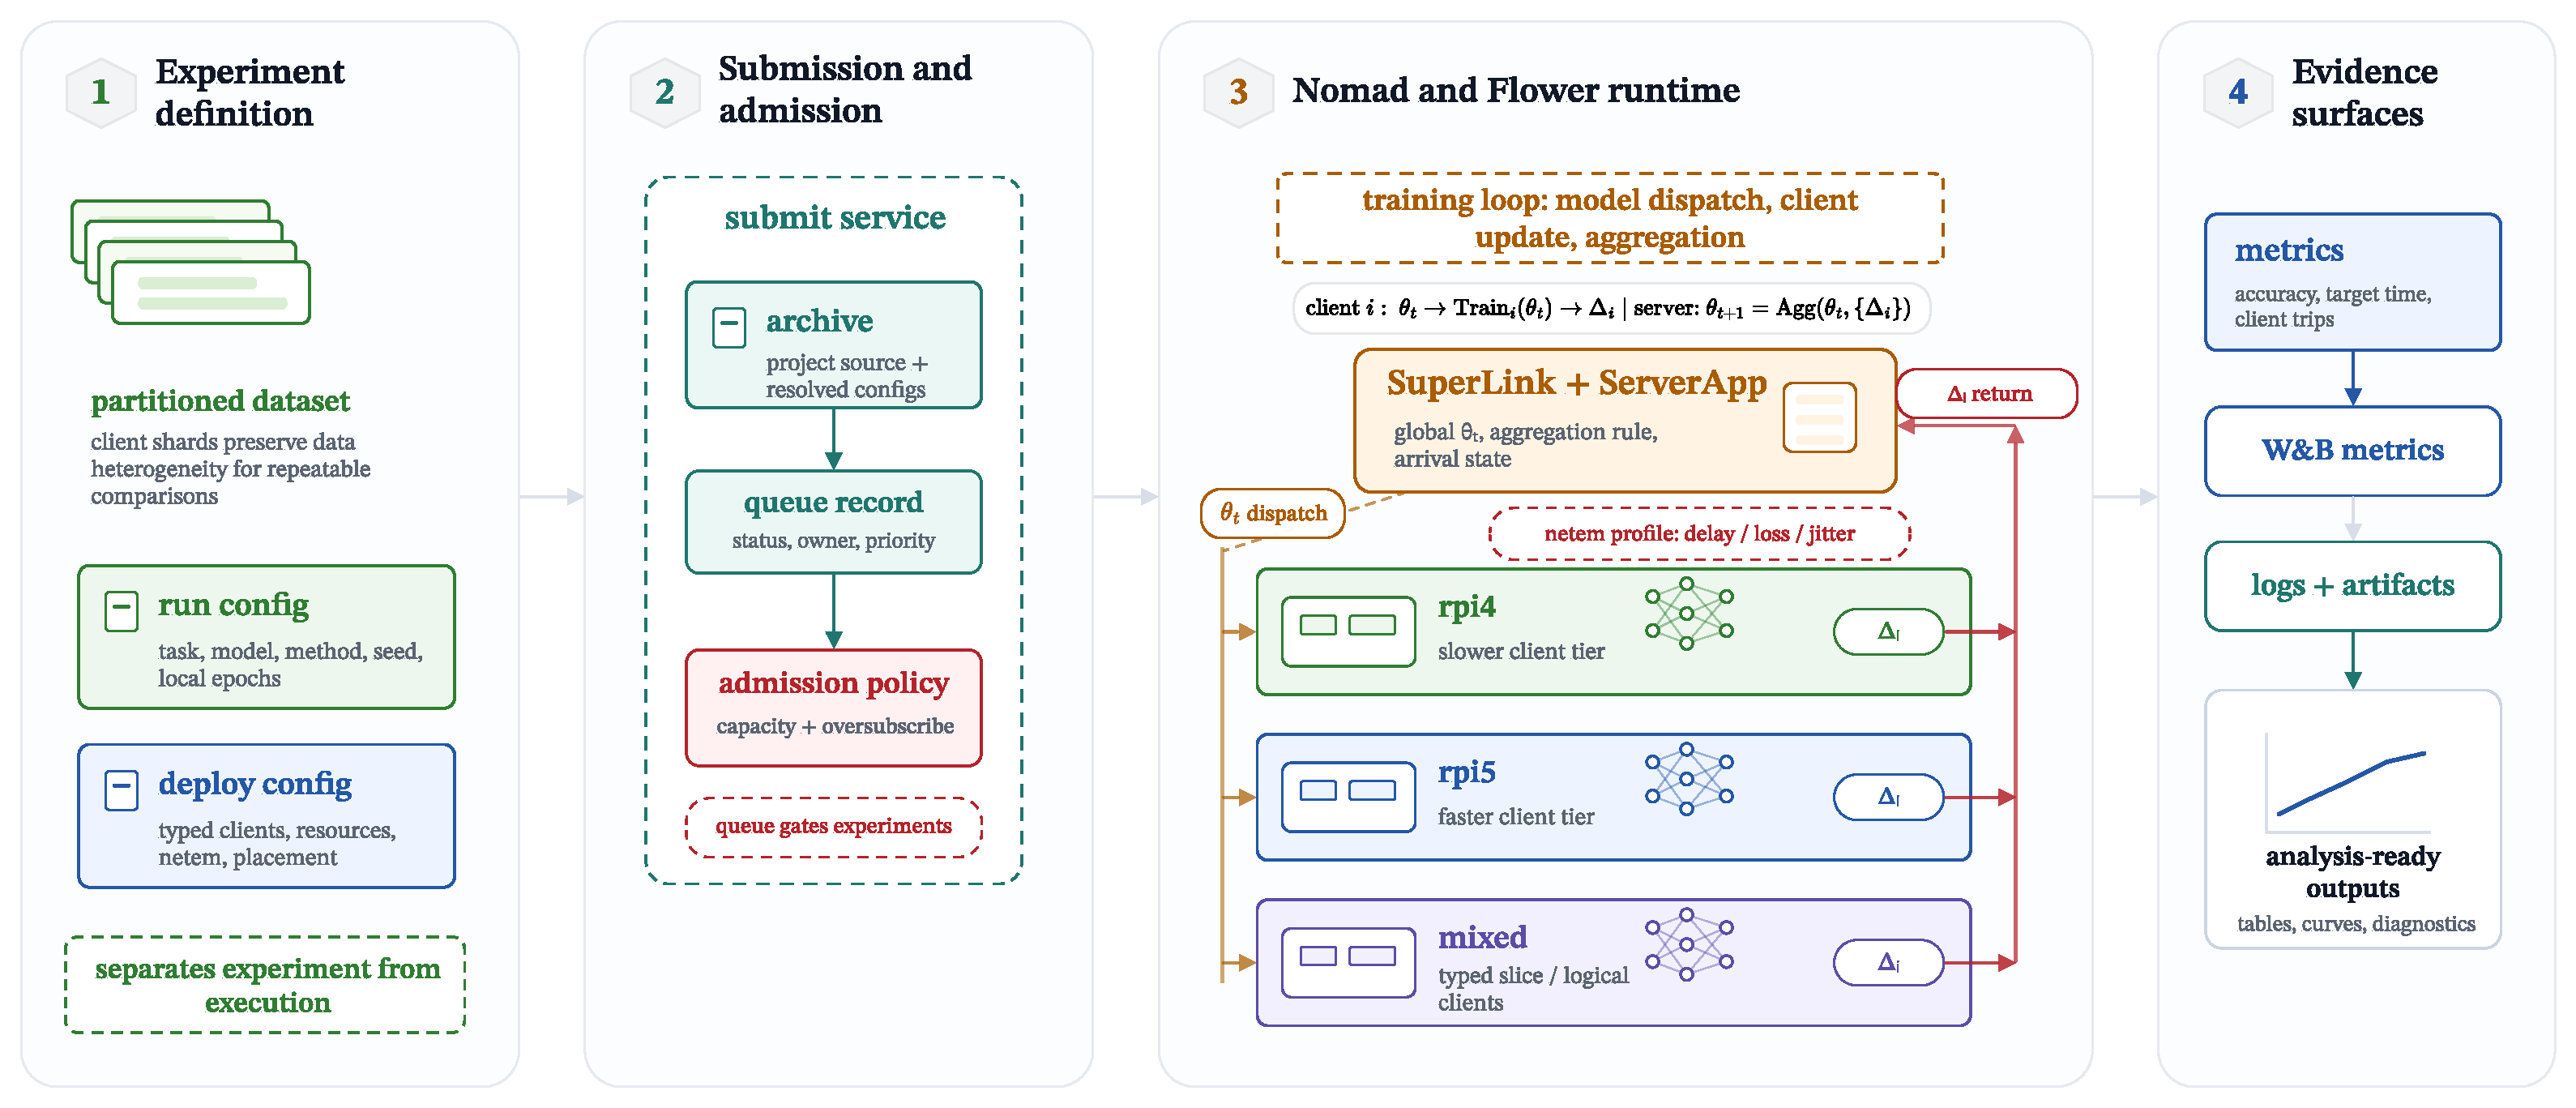
\includegraphics[width=\textwidth]{figures/remote_execution_lifecycle_clean.pdf}%
}
\caption{\textbf{Remote execution lifecycle.}}
\label{fig:remote_execution_lifecycle}
\end{figure}

The request records the Flower project, workload choices, deployment choices, and CLI overrides. The uploaded bundle makes it executable away from the developer machine. The \implterm{paletteGreen}{queue} stores the run persistently; admission checks typed capacity and placement constraints; and the \implterm{paletteGreen}{submit runner} invokes the deployment path: build or select the SuperExec image, render Nomad jobs, configure the Flower federation, and start \texttt{flwr run}. Metrics, \implterm{gray}{structured artifacts}, and \implterm{gray}{logs} then become evaluation evidence.

\FloatBarrier
\subsection[Submission interface]{Submission interface \impltaghead{implcomp:request}{paletteGreen}{cli}}

The \implterm{paletteGreen}{submit interface} is the user-facing control surface for remote experiments. \texttt{fedctl submit run} creates the submission; companion commands inspect status, logs, inventory, and results, and can cancel or purge terminal records. See the website \href{http://fedctl.cl.cam.ac.uk/help\#reference}{\underline{command reference}} (accessible via CL network) for the full command set.

For dissertation experiments, the typical launch form passes a Flower project, a run config \runconf, and a deploy config \deployconf:

\begin{codeblock}{bash}
fedctl submit run <flower-project> \
  --run-config <run-config> \
  --deploy-config <deploy-config>
\end{codeblock}

\paragraph{Request capture.}
The \implterm{paletteGreen}{CLI} inspects the Flower project, resolves the configs, applies overrides such as seed or run name, and records the reconstructed user-facing command.

\paragraph{Transport and executable environment.}
As part of creating a submission, the CLI uploads the project and resolved configuration material needed by the remote runner. The request can then execute from the submit node without depending on the developer machine. Transient build products and machine-local state are excluded from the bundle.

The \implterm{paletteGreen}{submit runner} \submitrunner{} builds or reuses the SuperExec image stored in the \implterm{paletteGreen}{registry} \regtag{}. When possible, the image tag is derived from the build context, Dockerfile, and Flower version, so identical inputs are reused across seed and method sweeps.

\FloatBarrier
\subsection[Queued admission and dispatch]{Queued admission and dispatch \impltaghead{implcomp:request}{paletteGreen}{svc}\impltaghead{implcomp:substrate}{fedstalebrown}{cluster}}
\label{sec:impl_queued_admission}

The \implterm{paletteGreen}{submit service} separates an experiment batch into persistent records and dispatch decisions. A \implterm{paletteGreen}{queue record} stores identity, artifact, runner arguments, priority, status, job mapping, and logs. A dispatcher reconciles queued records with live \implterm{fedstalebrown}{Nomad state}; an admitted record becomes a submit-runner Nomad batch job that downloads the bundle, reports job mappings, and enters the deployment path. Figure~\ref{fig:queue_admission_dispatch} visualises this step.

\begin{figure}[!htbp]
\centering
\makebox[\textwidth][c]{%
  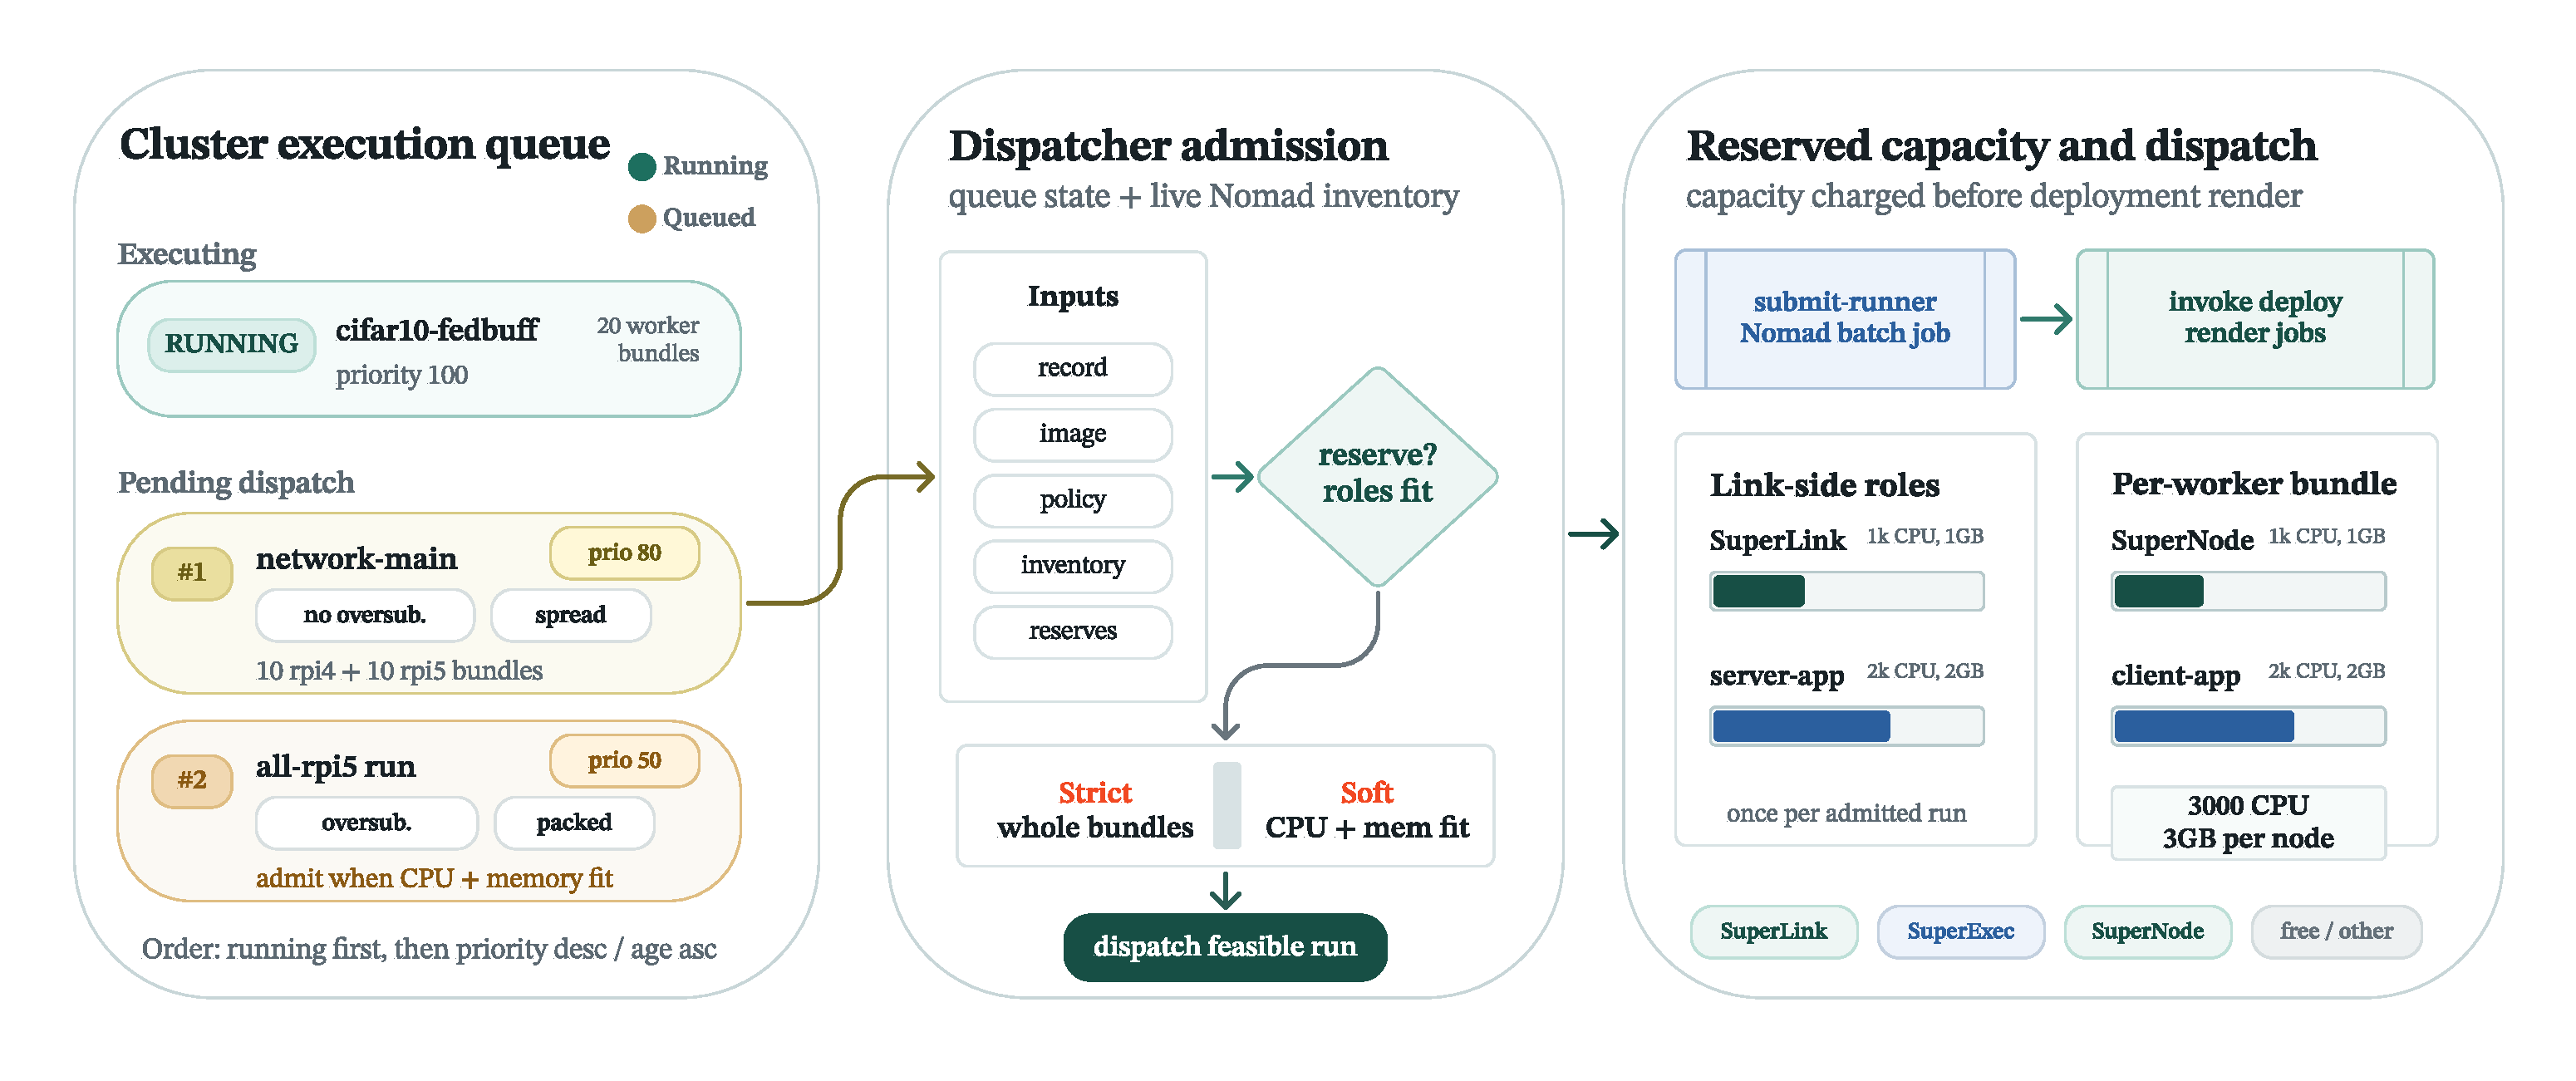
\includegraphics[width=1.08\textwidth]{figures/queue_admission_dispatch_clean.pdf}%
}
\caption{\textbf{Queued admission and dispatch path.}}
\label{fig:queue_admission_dispatch}
\end{figure}

% \begin{table}[!htbp]
% \centering
% \small
% \begin{tabularx}{\textwidth}{@{}>{\raggedright\arraybackslash}p{0.31\textwidth}>{\raggedright\arraybackslash}X@{}}
% \toprule
% \textbf{Admission input} & \textbf{How it is used} \\
% \midrule
% Submission record & Provides priority, namespace, submit image, artifact location, runner arguments, and current status. \\
% Runner arguments & Encode requested SuperNode counts, typed workers, and oversubscription policy. \\
% Deployment defaults & Provide resource reservations, node classes, and default placement policy when the request omits them. \\
% Nomad inventory & Supplies ready nodes, device type, node class, free CPU/memory, and visible allocations. \\
% Running submissions & Reserve capacity already consumed by active runs so later strict submissions do not collide with them. \\
% \bottomrule
% \end{tabularx}
% \caption{Inputs used by the submit-service dispatcher when deciding whether a queued run can be admitted.}
% \label{tab:submit_admission_inputs}
% \end{table}

\paragraph{Capacity and placement decision.}
Queueing is typed-capacity admission control. For strict deployments, the dispatcher accounts for whole typed worker bundles before dispatching, so a run requesting ten \texttt{rpi4} and ten \texttt{rpi5} workers waits until those devices are available. Placement can then either spread logical workers across distinct hosts, prefer spreading before reuse, or deliberately oversubscribe physical hosts.\footnote{These choices are controlled through the deploy config under \texttt{deploy.placement}, including \texttt{spread\_across\_hosts}, \texttt{prefer\_spread\_across\_hosts}, and \texttt{allow\_oversubscribe}.} Oversubscribed deployments use resource-based admission from live CPU and memory availability rather than exclusive device reservation, and the selected placement policy remains part of the recorded run state.

\FloatBarrier 
\subsection[Nomad rendering and service wiring]{Nomad rendering and service wiring \impltaghead{implcomp:deploy}{paletteGreen}{nomad}\impltaghead{implcomp:runtime}{paletteOrange}{roles}}

At this point, \texttt{fedctl} has a resolved deployment plan: the Flower roles to run, the device classes they should use, their resource reservations, and any network profiles. The \implterm{paletteGreen}{Nomad renderer} is the bridge from that plan to the cluster. It emits and submits the job specifications for SuperLink, SuperNodes, ServerApp, and ClientApps, starting the services first so their endpoints are discoverable before \texttt{flwr run} launches the application. Table~\ref{tab:nomad_flower_role_mapping} maps the Flower roles to the scheduler objects used in this deployment; Appendix~\ref{def:nomad} provides the Nomad vocabulary behind those objects.

\begin{table}[!htbp]
\centering
\small
{\renewcommand{\arraystretch}{1.18}
\begin{tabularx}{\textwidth}{@{}>{\raggedright\arraybackslash}p{0.16\textwidth}>{\raggedright\arraybackslash}p{0.28\textwidth}>{\raggedright\arraybackslash}X@{}}
\toprule
\textbf{Flower role} & \textbf{Nomad mapping} & \textbf{Purpose in the run} \\
\midrule
SuperLink & Link-class service job & Hosts the central Flower endpoints used by SuperNodes and the ServerApp. \\
SuperNodes & Service job with one task group per logical client & Provide client-side runtime endpoints; in \texttt{fedctl}, one endpoint is paired with each logical client and device placement. \\
ServerApp & Link-class service job & Runs the server application against the discovered SuperLink ServerApp endpoint. \\
ClientApp & One service job per logical client & Runs each client application against its paired SuperNode with client, device, and network metadata injected. \\
\bottomrule
\end{tabularx}
}
\caption{How the deployment renderer maps Flower runtime roles to Nomad jobs.}
\label{tab:nomad_flower_role_mapping}
\end{table}


% The control plane starts SuperLink first, then SuperNodes, then server-app and client-app SuperExec jobs. It writes the deployment manifest, configures the Flower project to use the remote federation, and invokes \texttt{flwr run <project> remote-deployment} with the materialized run config. Flower sees a normal remote deployment, while \texttt{fedctl} has already fixed placement, network, and service wiring.

\paragraph{Service discovery.}
Runtime addresses are injected through Nomad service definitions. SuperNodes discover the SuperLink service; the ServerApp receives the SuperLink ServerApp endpoint; and each ClientApp receives the corresponding SuperNode ClientApp endpoint. This makes the deployment robust to changing allocation IPs and ports across runs.

\paragraph{Runtime metadata.}
The renderer also injects experiment and placement metadata into the runtime. ClientApp containers receive the logical client index, device type, experiment identity, and, where strict placement is used, node identity. The research app \researchapp{} records this metadata with client metrics, which is what allows the evaluation to group training time, update share, and submodel quality by device class.

% Direct and queued runs converge on this downstream deployment path, so batch experiments and interactive debugging sessions exercise the same deployment code. The resulting operational state is exposed through the \implterm{gray}{submit-service UI and logs}, detailed in Appendix~\ref{appendix:observability_submit_ui}.


\FloatBarrier
\section{Controlling Real Hardware Heterogeneity}
\label{sec:impl_heterogeneity_control}

Hardware heterogeneity is inherent in a real edge cluster, but it must be controlled to support meaningful experiments. \texttt{fedctl} makes each client's hardware class and network conditions explicit at deployment time. Device-aware placement assigns logical clients to hardware classes; network impairment applies controlled communication conditions.

\FloatBarrier
\subsection[Device-aware placement]{Device-aware placement \impltaghead{implcomp:dep}{darkblue}{dep}\impltaghead{implcomp:deploy}{paletteGreen}{nomad}\impltaghead{implcomp:substrate}{fedstalebrown}{cluster}}

Device-aware placement exposes hardware heterogeneity as a declarative deployment variable. A run specifies \implterm{darkblue}{typed SuperNodes}, where each type corresponds to a hardware class such as \texttt{rpi4} or \texttt{rpi5}. Figure~\ref{fig:device_placement} traces this topology request to the device-labelled metrics used in the evaluation.

\begin{figure}[!htbp]
\centering
\makebox[\textwidth][c]{%
  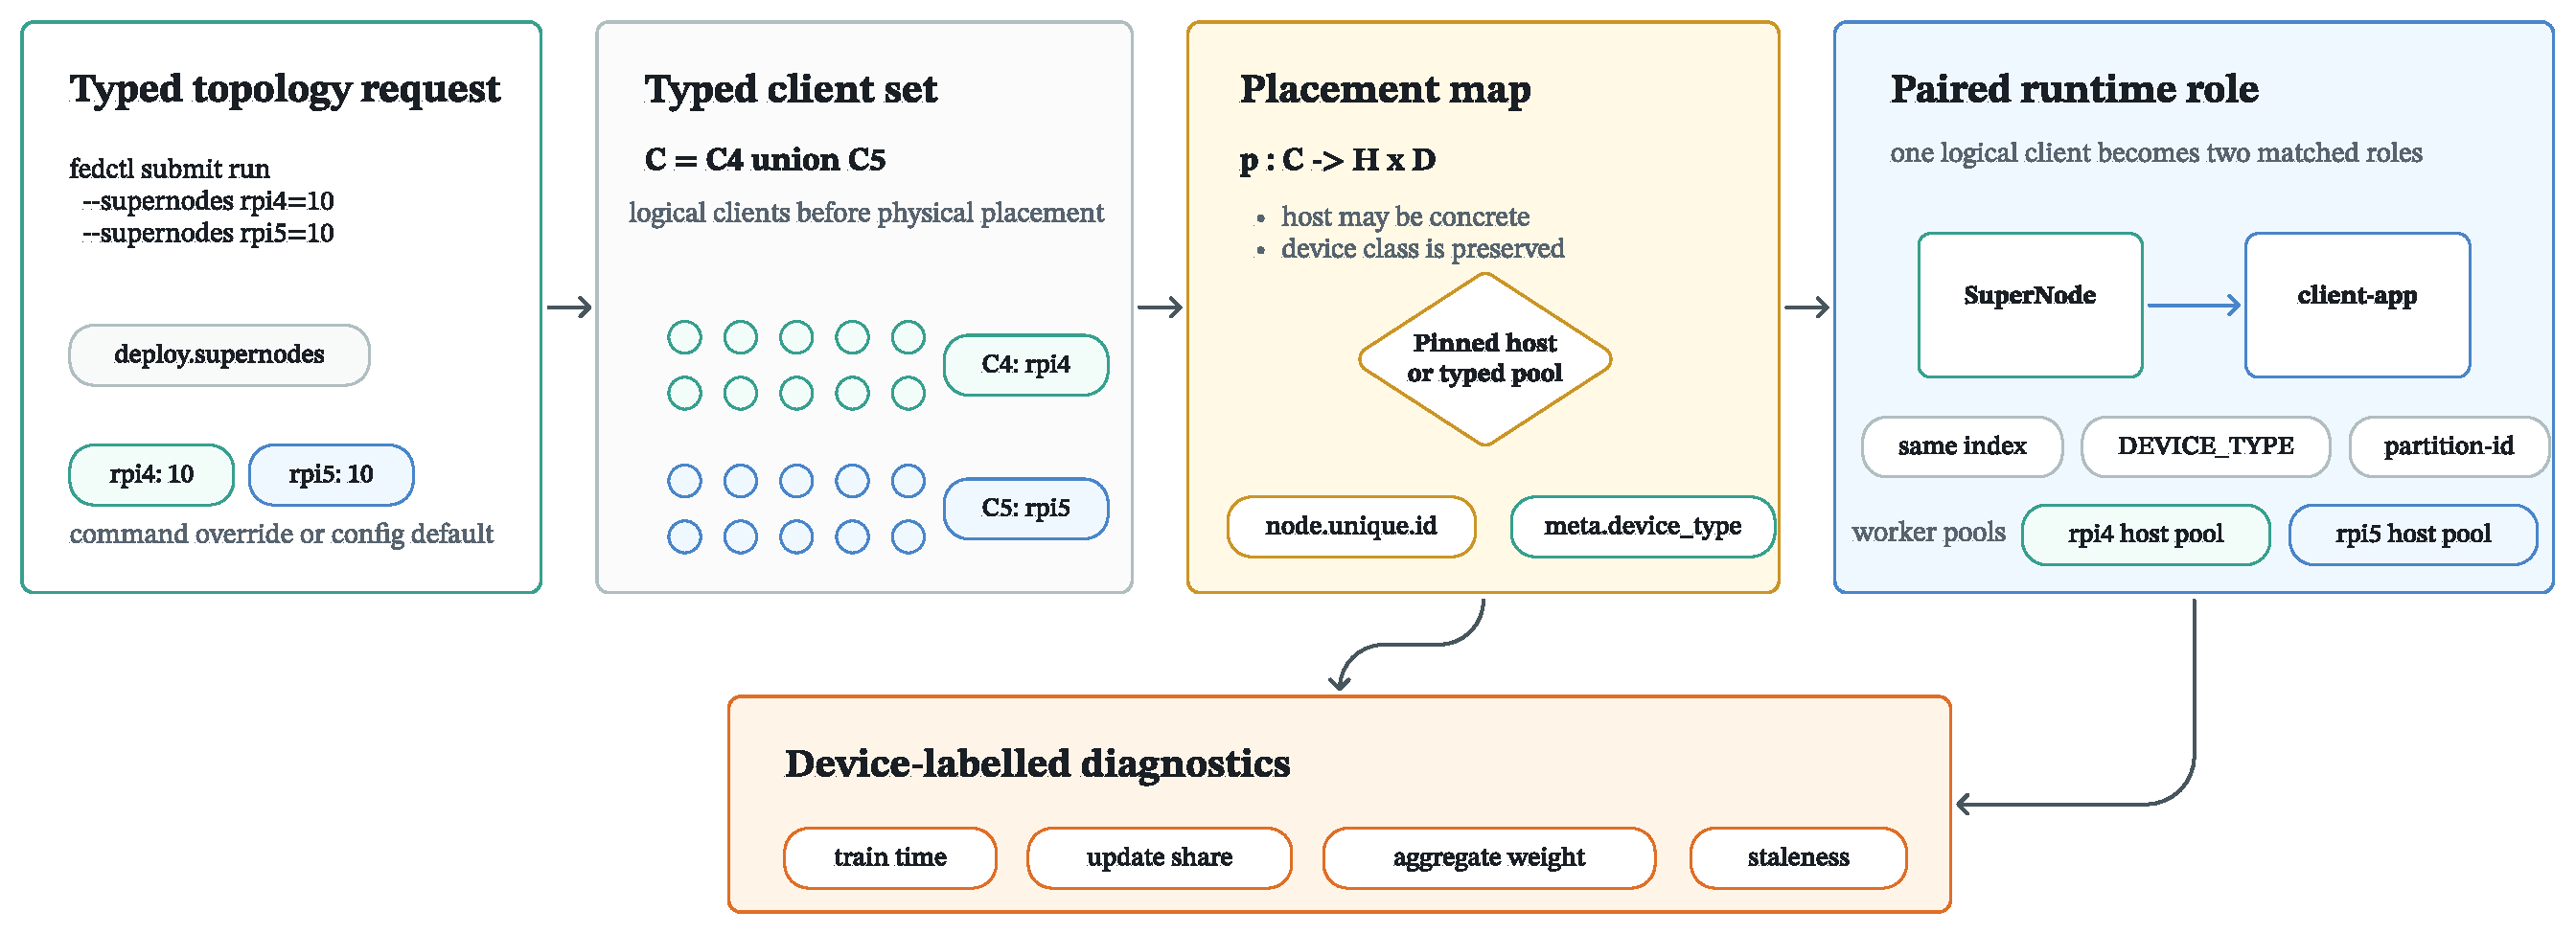
\includegraphics[width=\textwidth]{figures/device_placement_clean.pdf}%
}
\caption{\textbf{Device-aware placement and metadata flow.}}
\label{fig:device_placement}
\end{figure}

\paragraph{Typed SuperNodes.}
The interface is the \texttt{--supernodes} flag, which defines the logical topology as typed counts and overrides the deploy config \deployconf{} when present\footnote{If omitted, the same specification is read from \texttt{deploy.supernodes}. In both cases, the run records a typed SuperNode topology rather than a flat pool of interchangeable clients.}:
\begin{codeblock}{bash}
fedctl submit run <project>
  --supernodes rpi4=10, rpi5=10
\end{codeblock}


\paragraph{Deployment realisation.}
At deployment time, typed SuperNodes are mapped onto physical nodes by matching the requested type to \implterm{fedstalebrown}{Nomad node metadata}. Placement can be strictly pinned, constrained by device class, or expressed as a soft affinity. \footnote{It is enforced either by pinning to \texttt{node.unique.id} or by constraining \texttt{meta.device\_type}.}

\paragraph{Execution pairing.}
Each typed SuperNode is realised as a paired runtime: a Flower SuperNode communication endpoint and a corresponding client execution job. The pair shares a device-class constraint and a common instance index, so each logical SuperNode corresponds to exactly one communication endpoint and one execution context.

\paragraph{Evaluation linkage.}
Device type and instance identity are exposed to the application via environment variables, and are recorded with client metrics. This links deployment to evaluation: compute-heterogeneity experiments assign different model rates to \texttt{rpi4} and \texttt{rpi5}, while diagnostics such as training time, update share, aggregation weight, and staleness are analysed by device class.

\FloatBarrier
\subsection[Network impairment]{Network impairment \impltaghead{implcomp:dep}{darkblue}{dep}\impltaghead{implcomp:deploy}{paletteGreen}{nomad}}

Network impairment exposes communication heterogeneity as a deployment variable rather than a property of the FL method implementation. The deploy config \deployconf{} assigns a named impairment profile to each logical SuperNode. When a profile is active, \texttt{fedctl} renders the corresponding SuperNode task so that \texttt{flower-supernode} starts through a generated wrapper. The wrapper installs Linux traffic-control rules, verifies the resulting configuration, and then executes the normal SuperNode process. The research application and aggregation code therefore observe the same Flower runtime interface, while the deployment layer controls the network path.

\texttt{netem} is Linux's network-emulation facility for adding delay, jitter, packet loss, and bandwidth shaping; Appendix~\ref{def:network_evidence} gives the short definition used in this dissertation. Figure~\ref{fig:network_impairment} summarises the path from profile definition to logical assignment, Nomad rendering, wrapper setup, and ingress/egress enforcement.

\begin{figure}[!htbp]
\centering
\makebox[\textwidth][c]{%
  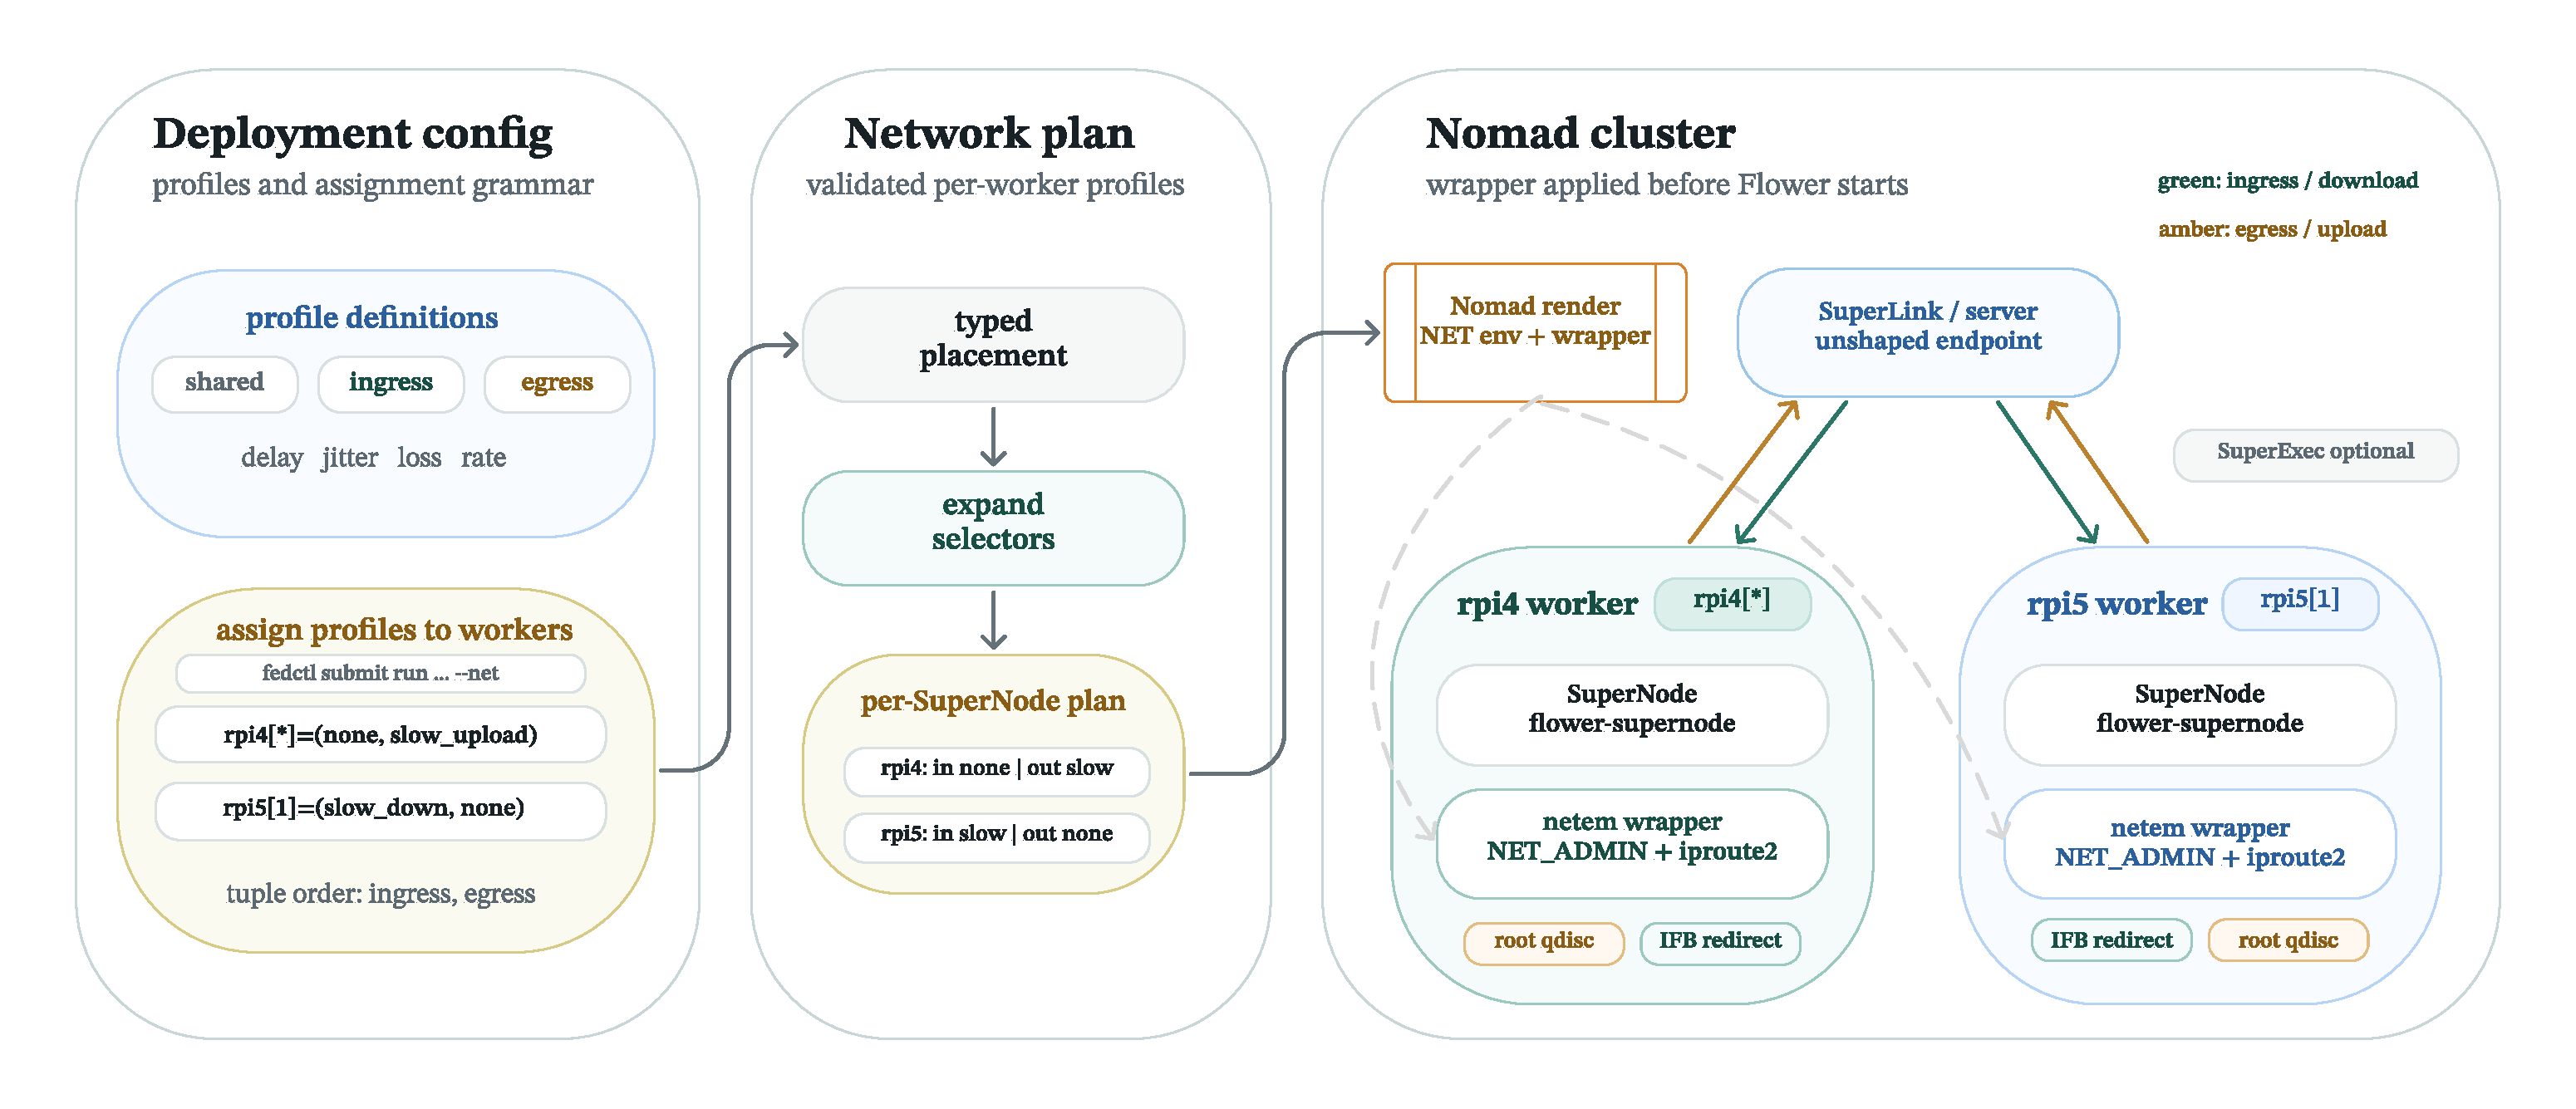
\includegraphics[width=1.08\textwidth]{figures/network_impairment_clean.pdf}%
}
\caption{\textbf{Network profile resolution and enforcement.}}
\label{fig:network_impairment}
\end{figure}

\paragraph{Profiles and assignment.}
A network profile is a named collection of traffic-shaping parameters consumed by the wrapper; \hyperlink{example:concrete-deploy-config}{\underline{the earlier deploy-config example}} gives one \texttt{mild} profile. Profiles may be symmetric or direction-specific, with \texttt{default\_profile} supplying the fallback when no explicit assignment is given. Assignments are resolved after typed placement, so selectors such as \texttt{rpi4[*]} or \texttt{rpi5[1]} refer to logical SuperNodes rather than physical hostnames. Direction-specific mappings use the tuple order \texttt{(ingress, egress)}, and the submit-time \texttt{--net} flag can override the deploy-config default.

\begin{table}[!htbp]
\centering
\small
\renewcommand{\arraystretch}{1.12}
\begin{tabularx}{\textwidth}{@{}>{\raggedright\arraybackslash}p{0.26\textwidth}>{\raggedright\arraybackslash}X@{}}
\toprule
\textbf{Parameter} & \textbf{Effect in the rendered task} \\
\midrule
\texttt{delay\_ms} & Adds base latency using \texttt{netem delay}. \\
\texttt{jitter\_ms} & Adds variation around the configured base latency. \\
\texttt{loss\_pct} & Drops the configured percentage of packets. \\
\texttt{rate\_mbit} & Adds a token-bucket bandwidth cap before delay/loss rules. \\
\texttt{rate\_latency\_ms} & Sets the token-bucket latency bound used with \texttt{rate\_mbit}. \\
\texttt{rate\_burst\_kbit} & Sets the token-bucket burst size used with \texttt{rate\_mbit}. \\
\bottomrule
\end{tabularx}
\caption{Traffic-shaping parameters consumed by the network-impairment wrapper. The same fields can define symmetric profiles or separate ingress and egress profiles.}
\label{tab:impl_network_profiles}
\end{table}

\paragraph{Wrapper enforcement.}
At deployment time, \texttt{fedctl} validates the selected profiles, expands typed selectors, and renders each affected SuperNode task to run as \texttt{root} with Docker \texttt{NET\_ADMIN}. The task receives \texttt{NET\_*} variables and starts through the generated wrapper script. Egress impairment attaches \texttt{tc qdisc} rules directly to the task interface. Ingress impairment redirects packets through an \texttt{ifb} device before applying the same token-bucket and \texttt{netem} controls. The wrapper then \texttt{exec}s \texttt{flower-supernode}, so the deployed FL application continues to use the normal Flower interface.

% \paragraph{Experimental scope.}
% The reported network experiments apply impairment at the SuperNode role. This targets the communication path between logical clients and the Flower federation while keeping server and client application code unchanged. The same wrapper mechanism could also be enabled for ServerApp or ClientApp SuperExec roles, but those extensions are not used in the dissertation experiments.

\FloatBarrier
\section{Flower Application and Method Layer}
\label{sec:impl_flower_application}

The dissertation-specific FL logic is implemented in the \implterm{paletteOrange}{research app} \researchapp{}. It resolves run configs, constructs tasks and models, loads partitions, executes local client work, coordinates server-side methods, and records method-level outputs. Figure~\ref{fig:application_method_layer} shows the boundary between deployment metadata, shared server/client task code, and the evidence consumed by Chapter~\ref{chap:evaluation}.

\begin{figure}[!htbp]
\centering
\makebox[\textwidth][c]{%
  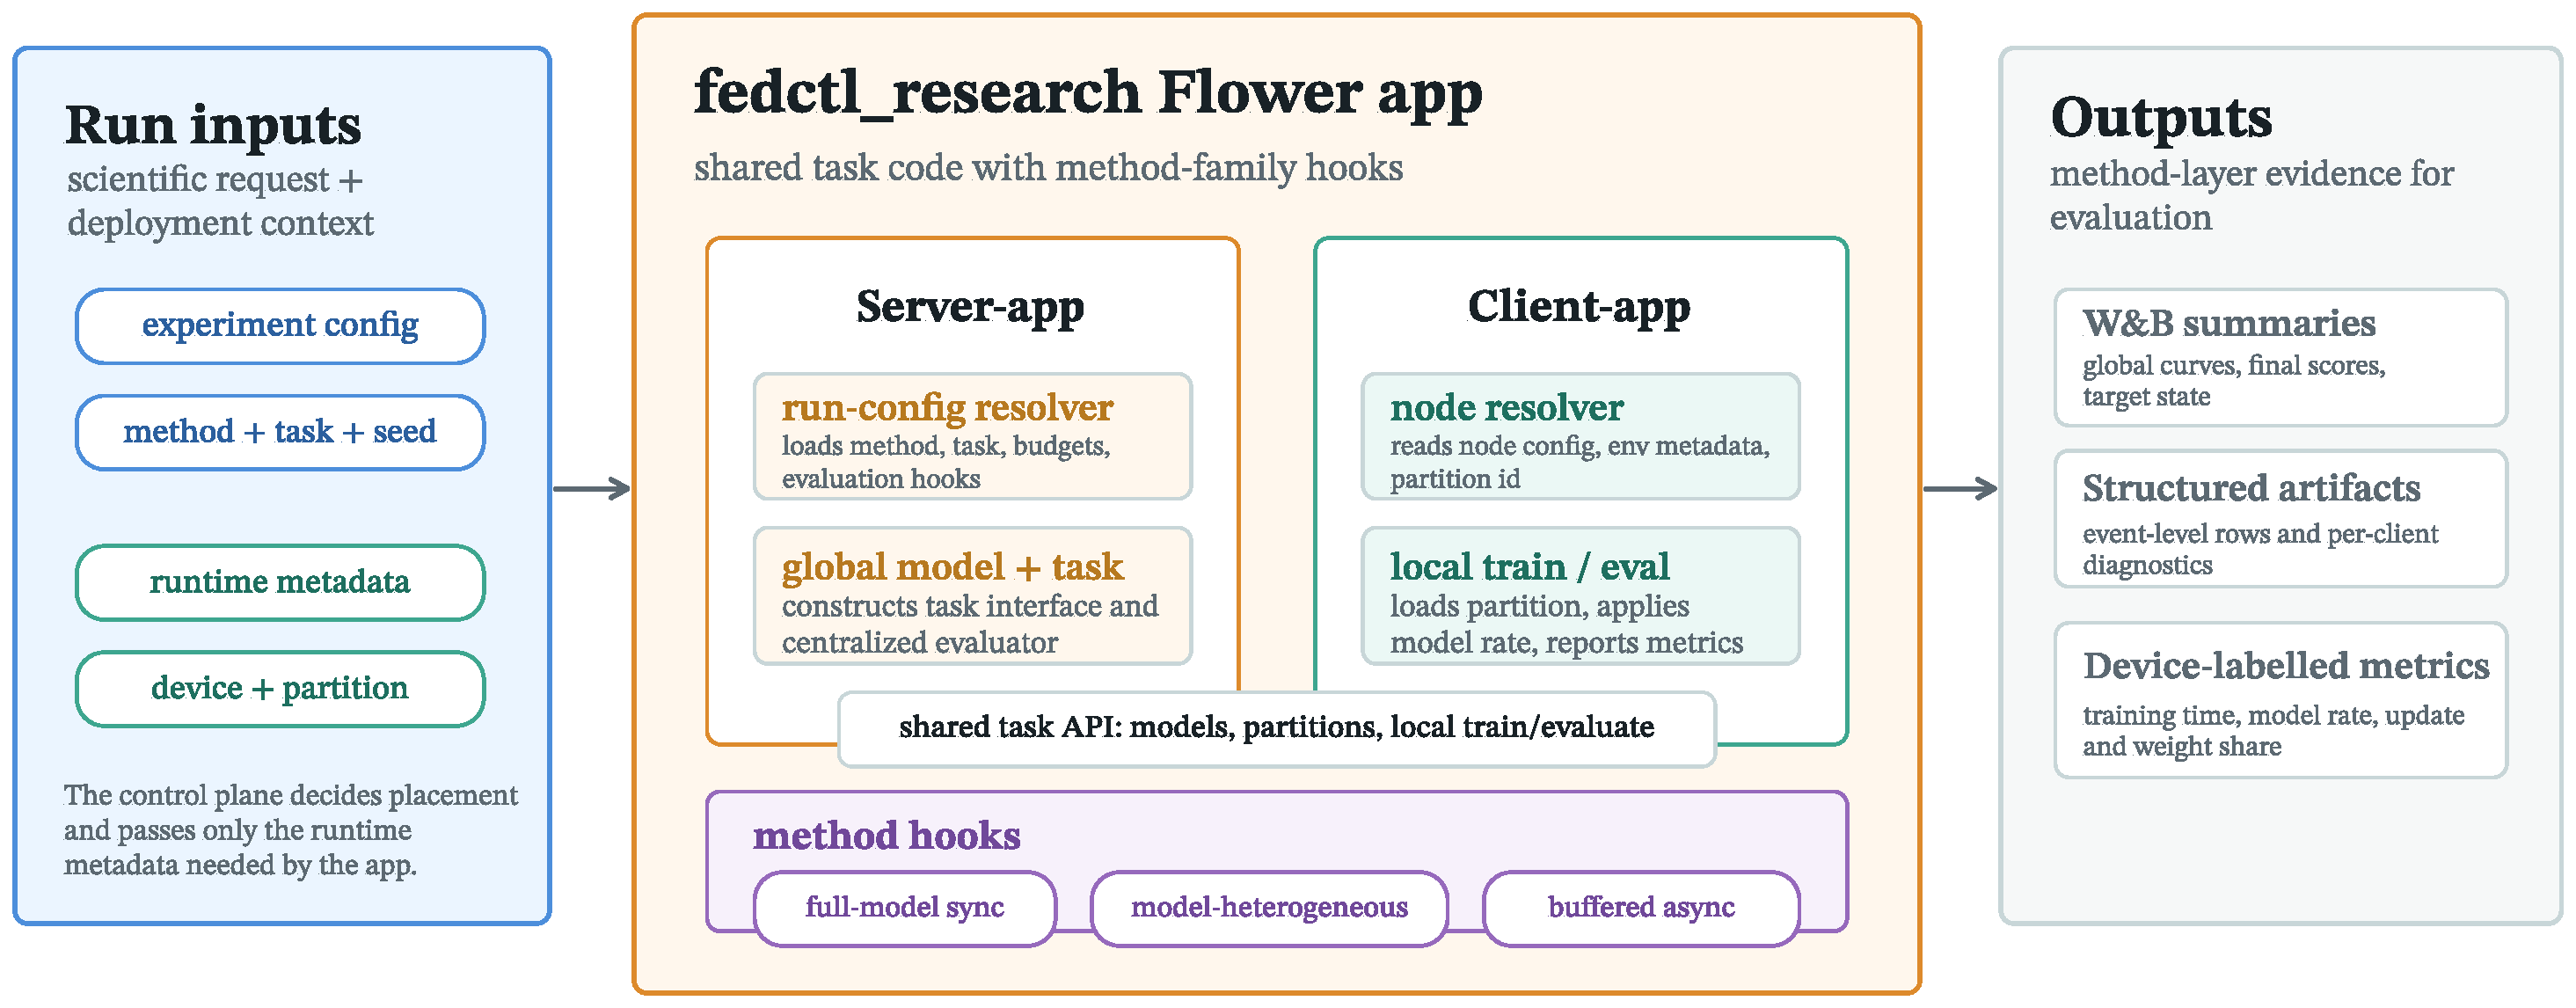
\includegraphics[width=\textwidth]{figures/application_method_layer.pdf}%
}
\caption{\textbf{Research application and method layer.}}
\label{fig:application_method_layer}
\end{figure}

\subsection[Research-app interface]{Research-app interface \impltaghead{implcomp:runtime}{paletteOrange}{app}}

The server and client entry points share one task interface. A run config selects the task, model, partitioner, method, optimizer settings, local budget, and evaluation path; the task implementation then supplies model construction, partition loading, local training, local evaluation, and centralized evaluation. Appendix~\ref{appendix:evaluation_tasks} summarises the evaluation datasets and task models instantiated through this interface.

Clients return updated parameters together with loss, example count, timing, throughput, device type, model rate, and partition identity. The server records target attainment, centralized evaluation, asynchronous staleness, accepted-update metadata, and method-specific diagnostics. This evidence path is what lets Chapter~\ref{chap:evaluation} relate accuracy, runtime, submodel quality, and slow-device influence back to the deployment choices fixed by \texttt{fedctl}.

\FloatBarrier
\subsection{Implemented method families}

The method layer implements the families evaluated in Chapter~\ref{chap:evaluation}. Chapter~\ref{chap:related_work} gives prior-method context, and Appendix~\ref{appendix:algorithms} gives unified pseudocode; here the emphasis is on the implementation distinctions needed for deployed experiments.

\paragraph{Full-model synchronous training.}
\texttt{FedAvg} is the full-model synchronous baseline. The server broadcasts the same global model to selected clients, waits for the configured replies, and aggregates returned models by example count.

\paragraph{Submodel training.}
\texttt{HeteroFL}, \texttt{FedRolex}, and \texttt{FIARSE} share one partial-training pipeline: select the client-visible parameter subset, train locally, scatter returned updates back into the global model, and aggregate only covered regions. They differ in the selection rule: fixed nested slices for \texttt{HeteroFL}, rolling windows for \texttt{FedRolex}, and sparse importance masks for \texttt{FIARSE}. \texttt{FIARSE} follows the paper's sparse-mask training mechanism, but executes those masks through dense PyTorch kernels on worker CPUs, so improved submodel quality does not necessarily translate into measured wall-clock speedup.

\paragraph{Buffered asynchronous training.}
\texttt{FedBuff} and \texttt{FedStaleWeight} use a custom buffered asynchronous server loop so the implementation can control in-flight concurrency, buffering, staleness, and accepted-update logging. \texttt{FedStaleWeight} changes only the buffer weighting rule, using the stale-aware weighting described in Section~\ref{sec:fedstaleweight_related}. The server records both update share and weight share, separating arrival frequency from aggregate influence.

\paragraph{Asynchronous submodel FL.}
\texttt{FedCover} combines the buffered asynchronous loop with HeteroFL-style nested submodels. Each reply carries its model rate and trained parameter slice, allowing the server to scatter the returned delta into the global parameter space and measure which parameters were covered. Section~\ref{sec:fedcover_impl} introduces the resulting coverage-aware aggregation algorithm.

\FloatBarrier
\section{\texttt{FedCover}: Coverage-Aware Buffered Aggregation}
\label{sec:fedcover_impl}

This section defines \texttt{FedCover} for asynchronous submodel FL, the setting introduced in Section~\ref{sec:async_submodel_related}. The base path combines \texttt{FedBuff}-style buffering with \texttt{HeteroFL}-style nested slicing; \texttt{FedCover} keeps that path and adds only a capped inverse-coverage correction to each aggregated parameter delta.

\paragraph{Buffered submodel replies.}
At server step \(s\), let \(\mathcal{B}_s\) be the accepted buffer, let \(\alpha_i\) be the stale-update weight for reply \(i\), and let \(I_i\) be the submodel parameter set trained by that reply. The shared asynchronous sign convention is \(\Delta_i=w^{[v_i]}-\tilde{w}_i\), with local component \(\Delta_{i,j}\) defined when \(j \in I_i\).

\paragraph{Parameter-level coverage.}
The buffered partial-model delta for parameter \(j\) is
\[
    \bar{\Delta}_j^{[s]}
    =
    \sum_{i \in \mathcal{B}_s}
    \alpha_i \mathbf{1}[j \in I_i]\Delta_{i,j}.
\]
FedCover also measures the observed coverage mass,
\[
    c_j^{[s]} =
    \sum_{i \in \mathcal{B}_s}
    \alpha_i \mathbf{1}[j \in I_i].
\]
The weights \(\alpha_i\) are normalized over the accepted buffer, so \(0 \le c_j^{[s]} \le 1\). The coverage mass is the stale-weighted accepted mass whose submodel contains \(j\), not a count of buffered replies. Thus, under-covered parameters receive a smaller effective update even when the buffer itself is full.

\paragraph{Inverse-coverage gain.}
Figure~\ref{fig:fedcover_coverage_gain} illustrates coverage mass for one parameter and the resulting gain curve.

\begin{figure}[!htbp]
\centering
\begin{adjustbox}{max width=\textwidth}
\begin{tikzpicture}[
  font=\scriptsize,
  >=Latex,
  cell/.style={minimum width=1.06cm, minimum height=0.58cm, draw=gray!45, line width=0.3pt, align=center},
  covered/.style={cell, fill=paletteGreen!16, draw=paletteGreen!65!black, text=paletteGreen!35!black},
  missing/.style={cell, fill=gray!7, draw=gray!40, text=gray!60},
  note/.style={align=center, text=gray!75!black},
  paneltitle/.style={font=\small\bfseries, align=center}
]
  \node[paneltitle] at (2.55,3.85) {Accepted buffer for one parameter \(j\)};
  \node[note] at (2.55,3.42) {\(\sum_{i\in\mathcal{B}_s}\alpha_i=1\), but not every reply covers \(j\)};

  \node[anchor=east, font=\scriptsize\bfseries] at (-0.70,2.74) {reply};
  \node[anchor=east, font=\scriptsize\bfseries] at (-0.70,2.06) {\(\alpha_i\)};
  \node[anchor=east, font=\scriptsize\bfseries] at (-0.70,1.38) {covers \(j\)};

  \foreach \x/\name/\weight/\state in {
    0/{1}/0.25/yes,
    1.18/{2}/0.20/no,
    2.36/{3}/0.20/yes,
    3.54/{4}/0.20/no,
    4.72/{5}/0.15/yes
  } {
    \node[cell, fill=gray!3] at (\x,2.74) {\(i=\name\)};
    \node[cell, fill=gray!3] at (\x,2.06) {\(\weight\)};
  }
  \node[covered] at (0,1.38) {yes\\\(+0.25\)};
  \node[missing] at (1.18,1.38) {no\\\(+0\)};
  \node[covered] at (2.36,1.38) {yes\\\(+0.20\)};
  \node[missing] at (3.54,1.38) {no\\\(+0\)};
  \node[covered] at (4.72,1.38) {yes\\\(+0.15\)};

  \draw[->, line width=0.5pt, paletteGreen!80!black]
    (2.36,0.80) -- (2.36,0.24);
  \node[
    rounded corners=2pt,
    draw=paletteGreen!60!black,
    fill=paletteGreen!8,
    align=center,
    inner sep=4pt,
    minimum width=4.8cm
  ] at (2.36,-0.32)
    {\(c_j^{[s]}=0.25+0.20+0.15=0.60\)\\observed coverage mass};

  \draw[gray!35, line width=0.4pt] (6.35,-0.80) -- (6.35,4.05);

  \node[paneltitle] at (10.25,3.85) {Capped inverse-coverage gain};
  \node[note] at (10.25,3.42) {example: \(\gamma=0.5,\ \kappa_{\max}=2\), so \(c_{\mathrm{cap}}=\kappa_{\max}^{-1/\gamma}=0.25\)};

  \coordinate (origin) at (8.05,0.10);
  \draw[->, line width=0.45pt] (origin) -- (12.65,0.10);
  \draw[->, line width=0.45pt] (origin) -- (8.05,2.80)
    node[above, font=\scriptsize] {\(\kappa(c)\)};

  \foreach \cx/\lab in {0/{0},0.25/{\(c_{\mathrm{cap}}\)},0.60/{0.60},1/{1}} {
    \draw[gray!55] ({8.05+4.15*\cx},0.10) -- ({8.05+4.15*\cx},0.00);
    \node[below, font=\scriptsize] at ({8.05+4.15*\cx},0.09) {\lab};
  }
  \foreach \ky/\lab in {1/{1},1.29/{1.29},2/{2}} {
    \draw[gray!55] (8.05,{0.10+2.25*(\ky-1)}) -- (7.95,{0.10+2.25*(\ky-1)});
    \node[left, font=\scriptsize] at (7.91,{0.10+2.25*(\ky-1)}) {\lab};
  }

  \draw[gray!20, line width=0.25pt] (8.05,0.10) grid[xstep=0.83, ystep=0.5625] (12.20,2.35);
  \draw[paletteOrange!90!black, very thick]
    plot[domain=0:0.25, samples=2] ({8.05+4.15*\x},{0.10+2.25});
  \draw[paletteOrange!90!black, very thick]
    plot[domain=0.25:1, samples=70] ({8.05+4.15*\x},{0.10+2.25*(1/sqrt(\x)-1)});

  \draw[dashed, paletteGreen!80!black]
    ({8.05+4.15*0.60},0.10) -- ({8.05+4.15*0.60},{0.10+2.25*(1/sqrt(0.60)-1)});
  \draw[dashed, paletteGreen!80!black]
    (8.05,{0.10+2.25*(1/sqrt(0.60)-1)}) -- ({8.05+4.15*0.60},{0.10+2.25*(1/sqrt(0.60)-1)});
  \fill[paletteGreen!80!black] ({8.05+4.15*0.60},{0.10+2.25*(1/sqrt(0.60)-1)}) circle (1.8pt);
  \node[
    rounded corners=2pt,
    draw=paletteGreen!60!black,
    fill=paletteGreen!8,
    align=center,
    inner sep=3pt,
    anchor=west
  ] at (10.75,1.33) {\(c=0.60\)\\\(\kappa=0.60^{-0.5}=1.29\)};

  \node[align=center, text=gray!75!black] at (10.10,-0.50) {observed coverage mass \(c\)};
  \node[anchor=north west, align=left, text=gray!75!black] at (8.00,-0.78)
    {\(\kappa(c)=\min(\kappa_{\max},c^{-\gamma})\), applied only when \(c>0\)};
\end{tikzpicture}
\end{adjustbox}
\caption{FedCover converts partial-model coverage into an inverse-coverage gain. The left panel shows one accepted buffer in which parameter \(j\) is present in only three replies, giving \(c_j^{[s]}=0.60\). The right panel shows the corresponding gain curve for an illustrative hyperparameter choice; the flat region is the gain cap, not an additional coverage threshold.}
\label{fig:fedcover_coverage_gain}
\end{figure}

Under nested submodels, shared prefix parameters have high coverage mass, while outer blocks used only by larger model rates have lower coverage mass. The server converts coverage mass directly into a capped inverse-coverage gain,
\[
    \kappa_j^{[s]}
    =
    \min\!\left(\kappa_{\max}, (c_j^{[s]})^{-\gamma}\right)
    \quad \text{for } c_j^{[s]} > 0.
\]

\paragraph{Corrected server update.}
The server applies
\[
    w_j^{[s+1]}
    =
    w_j^{[s]} - \eta_s \kappa_j^{[s]}\bar{\Delta}_j^{[s]}
    \quad \text{when } c_j^{[s]} > 0,
\]
and leaves \(w_j\) unchanged when the buffer contains no update for that parameter. The correction only rescales parameters that appear in the accepted buffer; it does not impute updates for parameters with \(c_j^{[s]}=0\). Full coverage gives \(\kappa_j^{[s]}=1\); lower coverage increases the update by an inverse-coverage factor, with \(\gamma\) controlling the correction strength and \(\kappa_{\max}\) preventing excessive amplification. If all clients train the full model, \texttt{FedCover} reduces to ordinary buffered asynchronous aggregation; setting \(\gamma=0\) recovers the coverage-disabled asynchronous \texttt{HeteroFL} baseline.

\FloatBarrier
% \section{Repository Organisation}
% \label{sec:impl_repo_overview}

% Figure~\ref{fig:repo_overview} maps the implementation mechanisms to the repository.

% \begin{figure}[!htbp]
% \centering
% \begin{adjustbox}{max width=\textwidth}
% \begin{minipage}{0.92\textwidth}
% \footnotesize
% \renewcommand*\DTstyle{\ttfamily}
% \renewcommand*\DTstylecomment{\normalfont\scriptsize\color{gray}}
% \DTsetlength{0.2em}{1.0em}{0.25em}{0.35pt}{1.2pt}
% \dirtree{%
% .1 fedctl/.
% .2 \textcolor{darkblue}{src/fedctl/}\DTcomment{generic control plane}.
% .3 \textcolor{darkblue}{commands/}\DTcomment{CLI entry points}.
% .3 \textcolor{darkblue}{build/}\DTcomment{image construction and reuse}.
% .3 \textcolor{darkblue}{deploy/}\DTcomment{Nomad planning, rendering, placement, netem}.
% .3 \textcolor{darkblue}{submit/}\DTcomment{submit-runner and artifact reporting}.
% .2 \textcolor{paletteGreen}{submit\_service/}\DTcomment{queue, dispatcher, UI, inspection APIs}.
% .2 \textcolor{fedrolexpurple}{apps/fedctl\_research/}\DTcomment{dissertation Flower app}.
% .3 \textcolor{fedrolexpurple}{src/fedctl\_research/}\DTcomment{tasks, methods, runtime, artifacts}.
% .3 \textcolor{fedrolexpurple}{run\_configs/}\DTcomment{Flower run-config definitions}.
% .3 \textcolor{fedrolexpurple}{deploy\_configs/}\DTcomment{deploy config presets used by fedctl}.
% .2 \textcolor{paletteOrange}{templates/}\DTcomment{Nomad and submit-runner templates}.
% .2 \textcolor{paletteOrange}{ansible/}\DTcomment{cluster provisioning}.
% .2 \textcolor{paletteOrange}{plot/}\DTcomment{figure/table generation}.
% .2 \textcolor{paletteOrange}{writeup/}\DTcomment{dissertation source and figures}.
% }
% \end{minipage}
% \end{adjustbox}
% \caption{\textbf{\texttt{fedctl} repository organisation.}}
% \label{fig:repo_overview}
% \end{figure}

% \texttt{src/fedctl} contains the \implterm{darkblue}{CLI and control-plane code} for packaging, building, deploying, submitting, and inspecting Flower workloads. \texttt{submit\_service} is the \implterm{paletteGreen}{queue, dispatcher, UI, and inspection layer}. \texttt{apps/fedctl\_research} is the \implterm{fedrolexpurple}{dissertation FL logic}: tasks, partitioners, methods, runtime helpers, run configs, deploy config presets, and result artifacts. \texttt{plot} and \texttt{writeup} support reproducible figures and thesis artifacts.

% Overall, the implementation turns heterogeneous worker hardware into an explicit experimental platform. The configuration split separates workload choices from execution conditions; the control plane packages and deploys runs reproducibly; typed placement and network profiles control compute heterogeneity and straggler-induced heterogeneity; and the research application emits the metrics used in Chapter~\ref{chap:evaluation}.
